% id: 135-c3
% book: 개념원리 중학 3-2 · 14 산점도와 상관관계
% section: 핵심문제 익히기
% figure: crop:fig-135-c3.png
% answer: ⑴ 3명 ⑵ 7명
% answer_source: 답지
% variant_level: 0 (원본 전사)
% 이 파일은 build.mjs 가 items.json 에서 만든다. 고칠 때는 items.json 을 고친다.
\smash{\raisebox{1.5mm}{\dmkichul{개념원리 중학 3-2 135쪽 확인 3}}}
\noindent\begin{minipage}[t]{0.58\linewidth}\vspace{0pt}\raggedright 오른쪽 그림은 재현이네 반 학생 15명의 수학 성적과 과학 성적을 조사하여 나타낸 산점도이다. 다음 물음에 답하시오.\end{minipage}\hfill\begin{minipage}[t]{0.4\linewidth}\vspace{0pt}\centering \setlength{\dmfigw}{94.2pt}\ifdim\dmfigw>\linewidth\setlength{\dmfigw}{\linewidth}\fi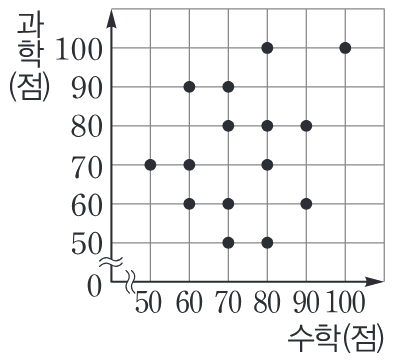
\includegraphics[width=\dmfigw]{figures/fig-135-c3.png}\end{minipage}\par
\dmsubprob{1} 수학 성적과 과학 성적의 차가 30점인 학생 수를 구하시오.
\dmsubprob{2} 수학 성적과 과학 성적의 차가 20점 이상인 학생 수를 구하시오.
